\documentclass[17pt,dvipdfmx]{beamer}
\usepackage{mypresentation}
\AtBeginShipoutFirst{\special{pdf:tounicode EUC-UCS2}}
\usepackage{minijs}

\setbeamerfont{title}{size=\HUGE{32},series=\bfseries,family=\rmfamily}
\setbeamerfont{frametitle}{size=\HUGE{24},series=\bfseries,family=\rmfamily}
\setbeamerfont{frametext}{size=\HUGE{20},series=\bfseries}
\setbeamertemplate{frametitle}[default][left]
\usefonttheme{professionalfonts}

\makeatletter
\define@key{beamerframe}{t}[true]{% top
  \beamer@frametopskip=.2cm plus .5\paperheight\relax%
  \beamer@framebottomskip=0pt plus 1fill\relax%
  \beamer@frametopskipautobreak=\beamer@frametopskip\relax%
  \beamer@framebottomskipautobreak=\beamer@framebottomskip\relax%
  \def\beamer@initfirstlineunskip{}%
}
\makeatother  

\setlength{\leftmargini}{12pt}
\setlength{\leftmarginii}{12pt}

\title{\mbox{My Experience in}\\ \mbox{TUG 2014}}% \\ 参加体験記}
\author{\mcfamily\bfseries 鹿野 桂一郎 \\
\small\bfseries \email{k16.shikano@gmail.com} \\ \twitter{golden\_lucky} }
\date{2014年11月8日}

\begin{document}

{\usebackgroundtemplate{
\includegraphics[height=\paperheight]{background.jpg}}%
\frame{\titlepage}
}

\begin{frame}[t]{What is TUG?}
  \bfseries\rmfamily
  \begin{columns}[t]
    \begin{column}{.4\textwidth}
      \vfill
      \hfill
\includegraphics[width=.9\textwidth]{tug.jpg}
    \end{column}
    \begin{column}{.7\textwidth}
    \begin{itemize}
      \item  The \TeX\ Users Group \\
      %\begin{itemize}
      %  \item The local user group of TeX users in North America
      %\end{itemize}
      %\item  TUGboat \\
      %\begin{itemize}
      %  \item The journal of the TUG
      %\end{itemize}
      %\item  Annual conference \\
      %\begin{itemize}
      %  \item held at Tokyo in 2013 \pause
      %  \item held at Portland in 2014
      %\end{itemize}
    \end{itemize}
    \vfill
    \end{column}
  \end{columns}
\end{frame}

\begin{frame}[t]{What is TUG?}
  \bfseries\rmfamily
  \begin{columns}[t]
    \begin{column}{.4\textwidth}
      \vfill
      \hfill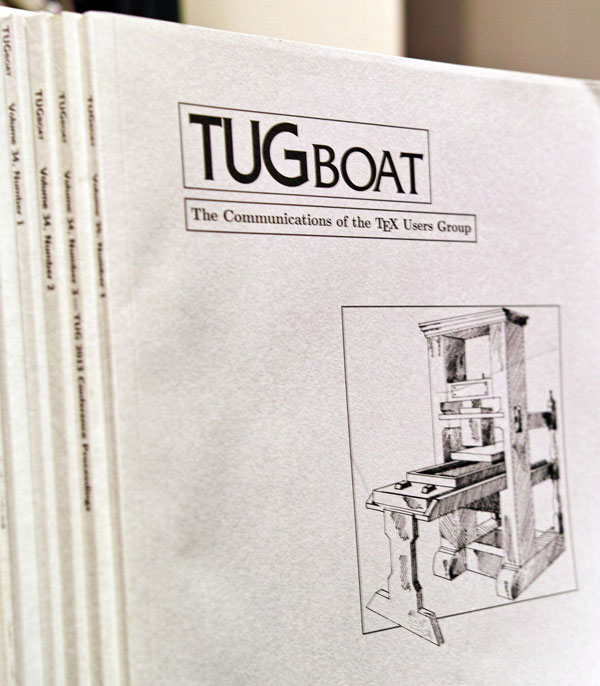
\includegraphics[width=.9\textwidth]{tugboat.jpg}
    \end{column}
    \begin{column}{.7\textwidth}
    \begin{itemize}
      \item  The \TeX\ Users Group \\
      %\begin{itemize}
      %  \item The local user group of TeX users in North America
      %\end{itemize}
      \item  TUGboat \\
      %\begin{itemize}
      %  \item The journal of the TUG
      %\end{itemize}
      %\item  Annual conference \\
      %\begin{itemize}
      %  \item held at Tokyo in 2013 \pause
      %  \item held at Portland in 2014
      %\end{itemize}
    \end{itemize}
    \vfill
    \end{column}
  \end{columns}
\end{frame}

\begin{frame}[t]{What is TUG?}
  \bfseries\rmfamily
  \begin{columns}[t]
    \begin{column}{.4\textwidth}
      \vfill
      \hfill
\includegraphics[width=.9\textwidth]{tug2013-color.jpg}
    \end{column}
    \begin{column}{.7\textwidth}
    \begin{itemize}
      \item  The \TeX\ Users Group \\
      %\begin{itemize}
      %  \item The local user group of TeX users in North America
      %\end{itemize}
      \item  TUGboat \\
      %\begin{itemize}
      %  \item The journal of the TUG
      %\end{itemize}
      \item  Annual conference \\
      \begin{itemize}
        \item held at Tokyo in 2013
        %\item held at Portland in 2014
      \end{itemize}
    \end{itemize}
    \vfill
    \end{column}
  \end{columns}
\end{frame}

\begin{frame}[t]{What is TUG?}
  \bfseries\rmfamily
  \begin{columns}[t]
    \begin{column}{.4\textwidth}
      \vfill
      \hfill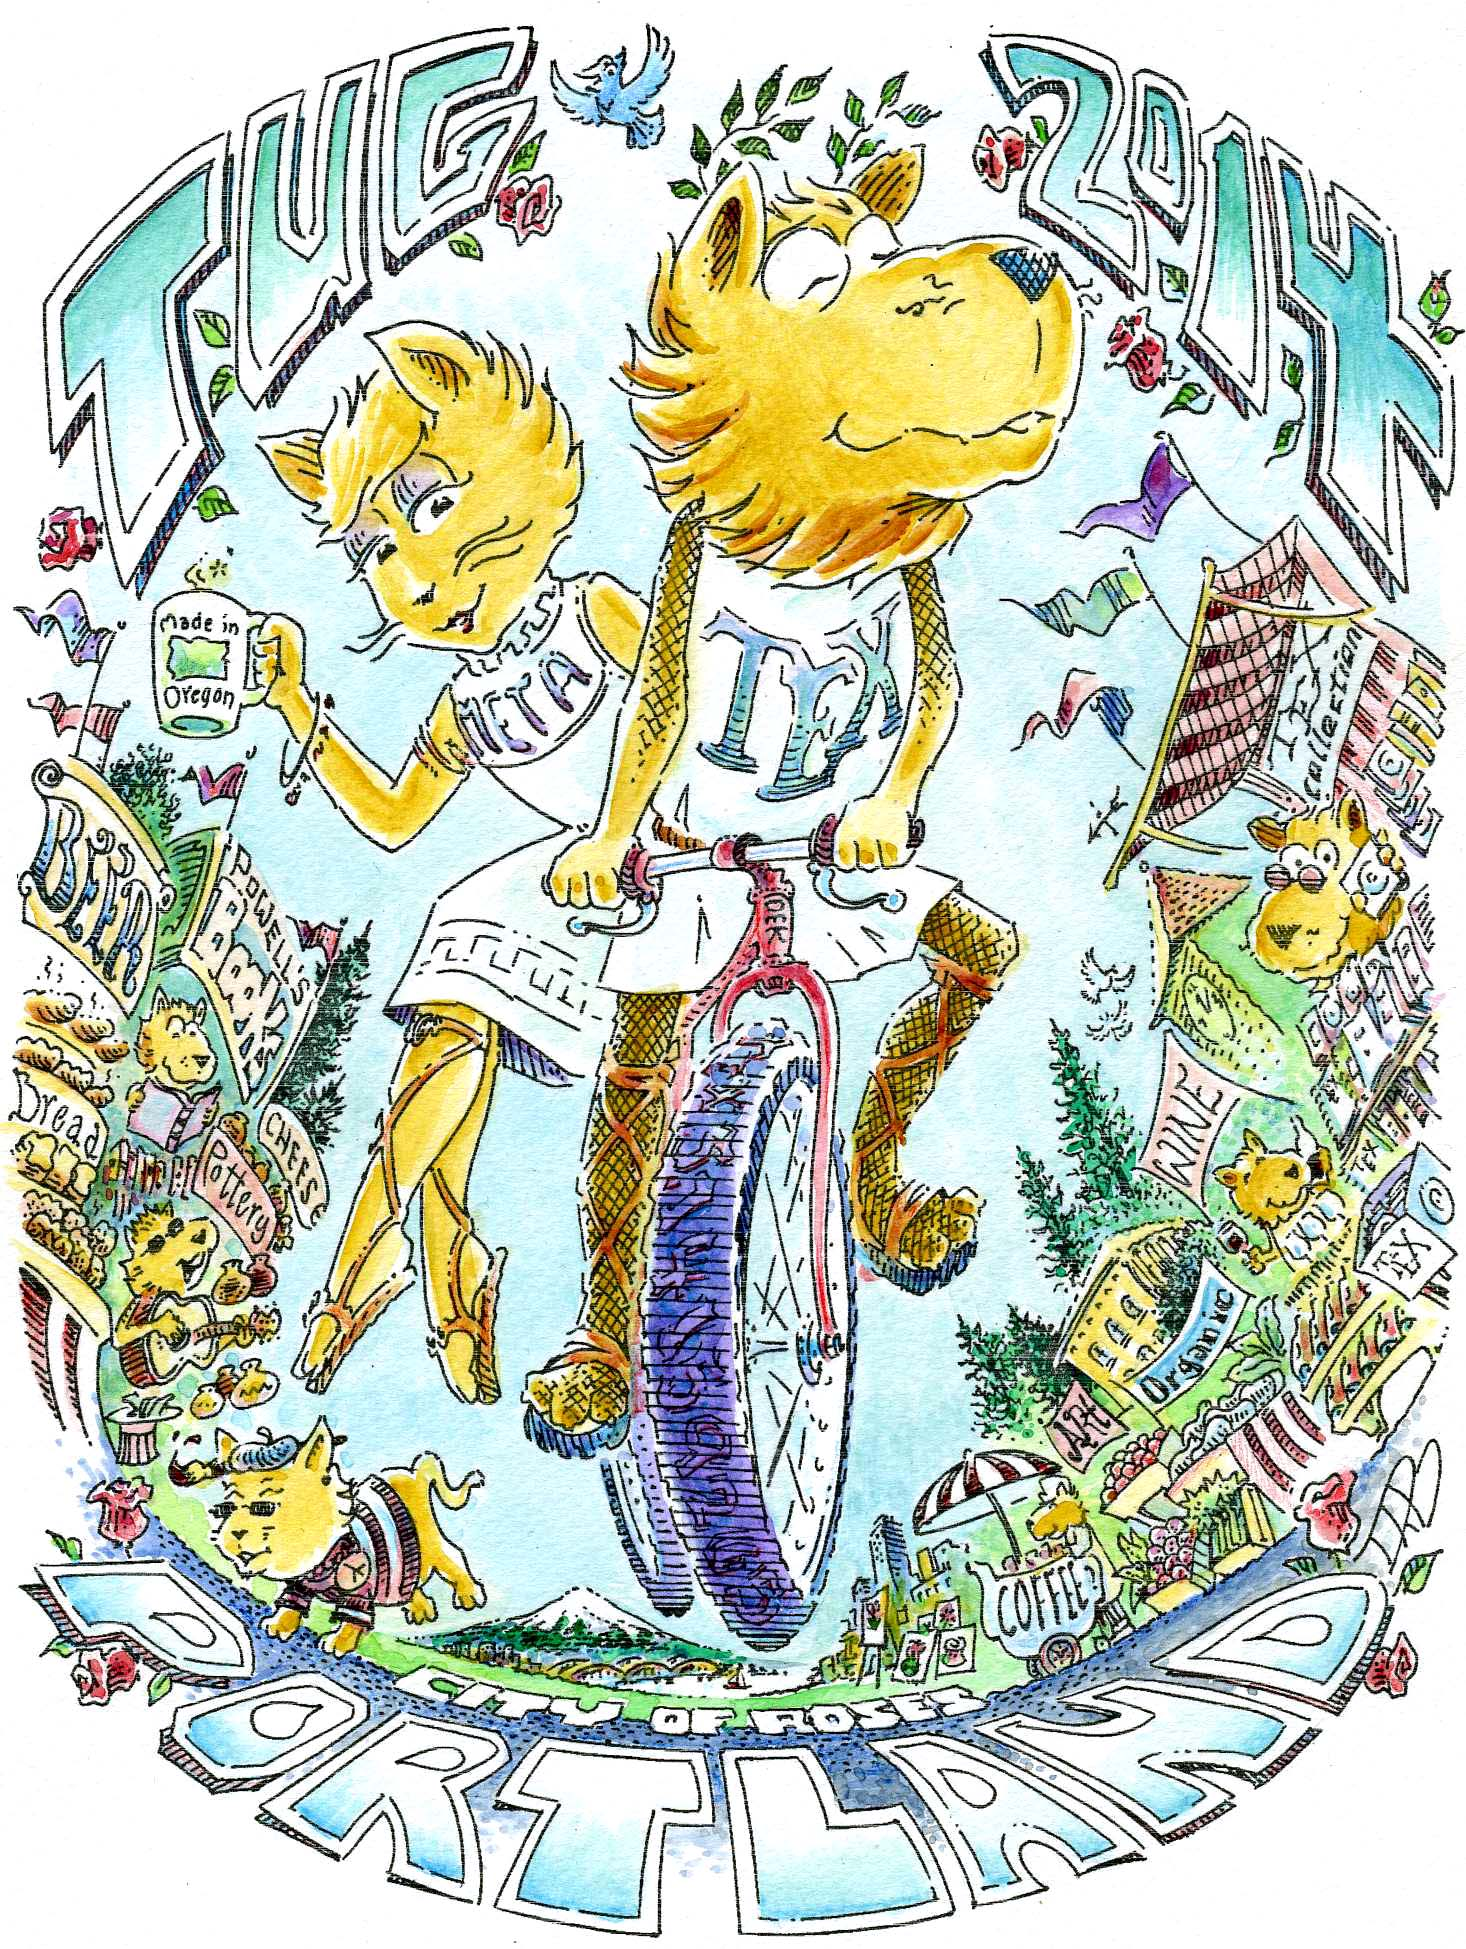
\includegraphics[width=.9\textwidth]{tug2014-color.jpg}
    \end{column}
    \begin{column}{.7\textwidth}
    \begin{itemize}
      \item  The \TeX\ Users Group \\
      %\begin{itemize}
      %  \item The local user group of TeX users in North America
      %\end{itemize}
      \item  TUGboat \\
      %\begin{itemize}
      %  \item The journal of the TUG
      %\end{itemize}
      \item  Annual conference \\
      \begin{itemize}
        \item held at Tokyo in 2013
        \item held at Portland in 2014
      \end{itemize}
    \end{itemize}
    \vfill
    \end{column}
  \end{columns}
\end{frame}

{\usebackgroundtemplate{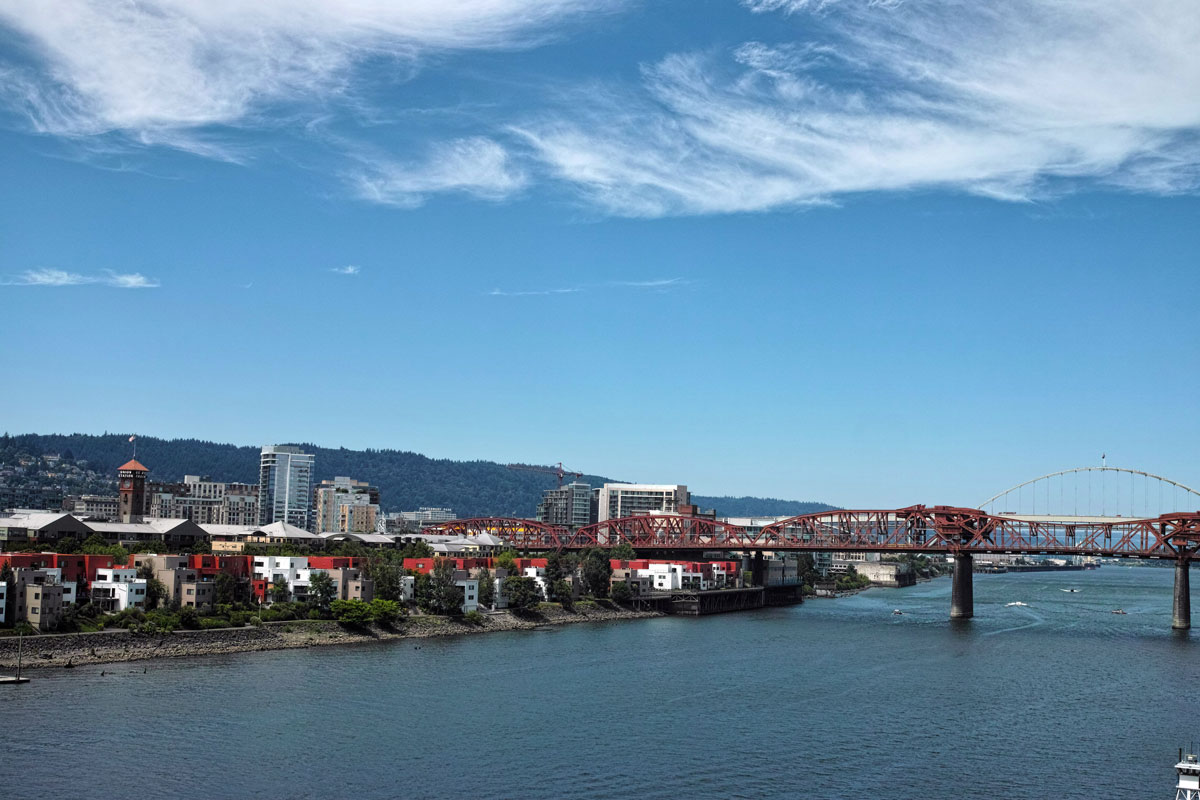
\includegraphics[height=\paperheight]{portland.jpg}}%
\begin{frame}[t]{{\color{black}What's Portland like?}}
  \bfseries\rmfamily
  \begin{itemize}
    \item Oregon, USA
    \item The home of the \TeX\ Users Group
    \item Known for roses, bikes, Willamette River, and brewers.
  \end{itemize}
  \vfill
\end{frame}
}

{\usebackgroundtemplate{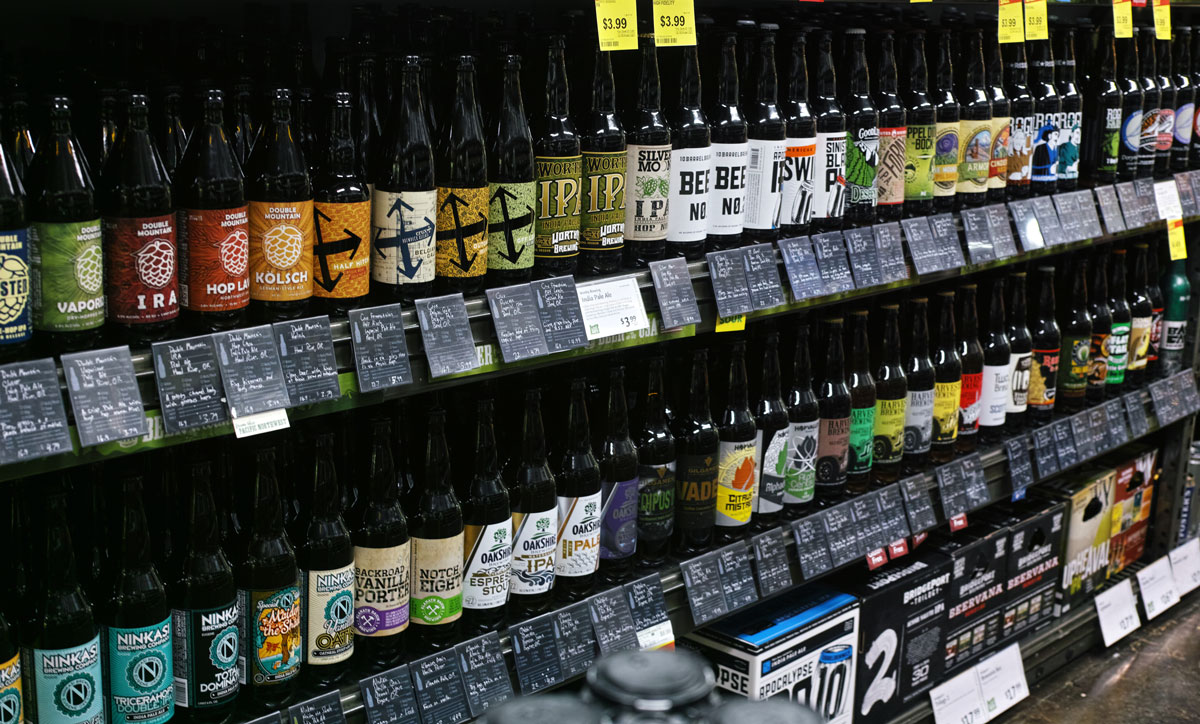
\includegraphics[height=\paperheight]{beer.jpg}}%
\frame
{
  \frametitle{{\HUGE{36}\color{white}Beer !}}
  \bfseries\rmfamily
  \begin{center}

  \end{center}
  \vfill
}}

\begin{frame}[t]{The Conference Place}
  \bfseries\rmfamily
  \begin{columns}[t]
    \begin{column}{.4\textwidth}
    \vfill
      \hspace*{11pt}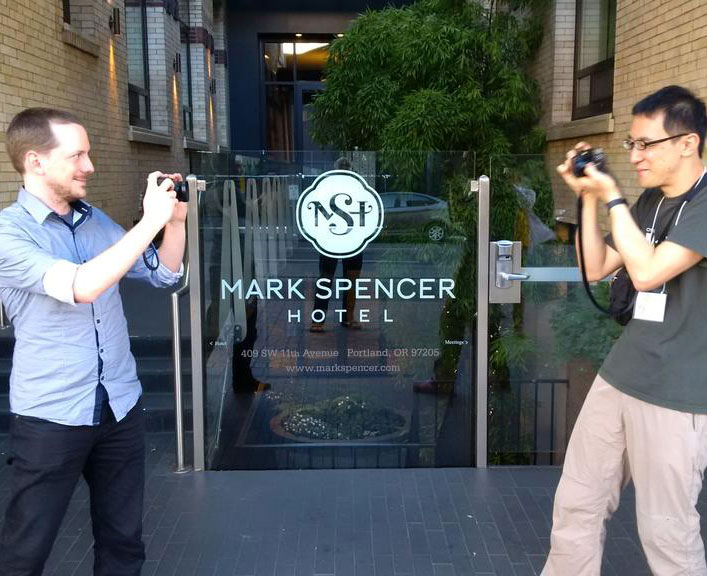
\includegraphics[width=.9\textwidth]{hotel3.jpg}
      {\vskip-.75\baselineskip\hbox to \textwidth{\hfill\HUGE{6}\copyright Pavneet Arora}}
    \end{column}
    \begin{column}{.7\textwidth}
    \begin{itemize}
      \item July 28 -- 30, 2014
      \item Mark Spencer Hotel in Downtown Portland
    \end{itemize}
    \end{column}
  \end{columns}
  \begin{columns}[t]
    \begin{column}{.6\textwidth}
      \setlength{\leftmargini}{24pt}
      \begin{itemize}
        \item Close to the world's biggest independent bookstore; Powell's
      \end{itemize}
    \end{column}
    \begin{column}{.4\textwidth}
    \vfill
      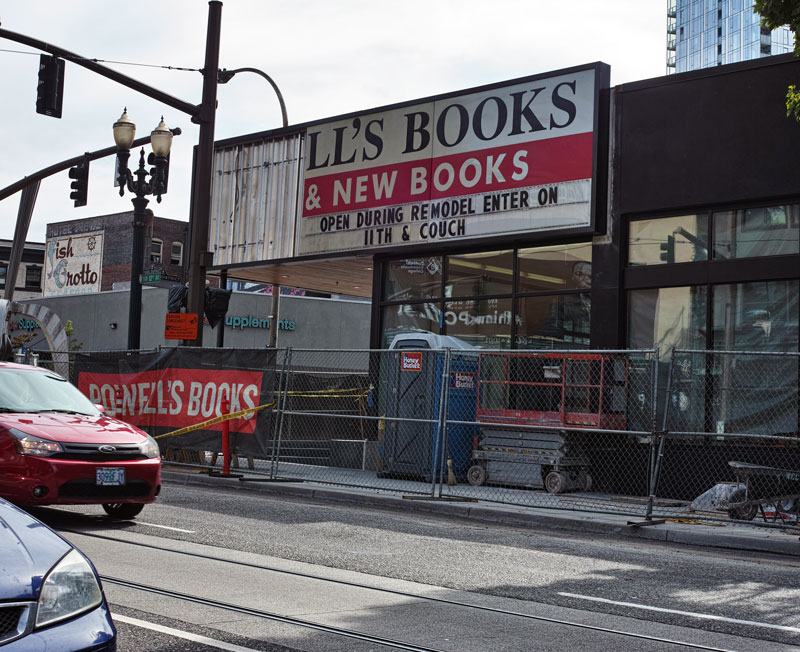
\includegraphics[width=.9\textwidth]{powells.jpg}
    \end{column}
  \end{columns}
\end{frame}

\begin{frame}[t]{Powell's Bookstore}
  \bfseries\rmfamily
  \begin{columns}[t]
    \begin{column}{.5\textwidth}
      \par\vspace*{0pt}\hspace*{30pt}
      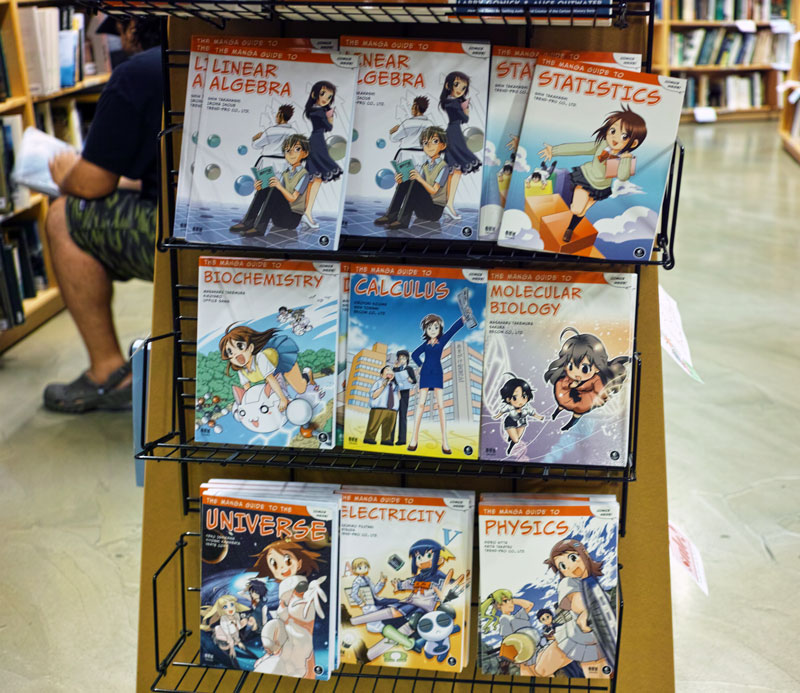
\includegraphics[width=.9\textwidth]{manga.jpg}
      \vfill
    \end{column}
    \begin{column}{.6\textwidth}
      \par\vspace*{40pt}\hspace*{-10pt}
      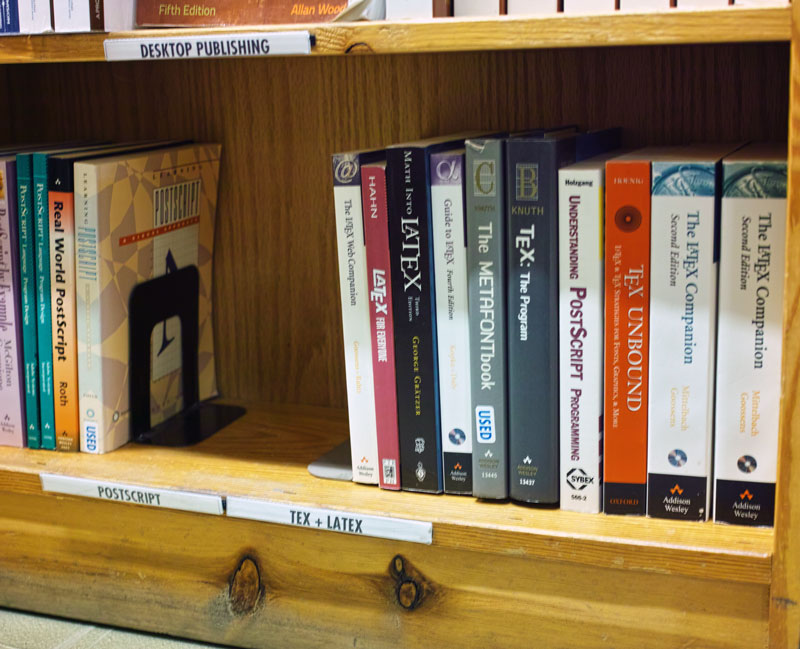
\includegraphics[width=.9\textwidth]{texbooks.jpg}
    \end{column}
  \end{columns}
\end{frame}

\begin{frame}[t]{Variety of Presentations}
  \bfseries\rmfamily
  \begin{itemize}
    \item 32 presentations / 56 participants \\
    \begin{itemize}
      \item Introducing \TeX-related tools
      \item ``What I've done using \TeX''
      \item Bringing up an idea on typesettings and documentations
    \end{itemize}
  \item You can see the whole program at\\[-5pt] 
  \hspace*{-2pt}\scalebox{0.9}[1]{\small{\url{https://tug.org/tug2014/program.html}}}
  \item You can see some articles at\\[-5pt] 
  \hspace*{-2pt}\scalebox{0.7}[1]{\small{\url{https://tug.org/TUGboat/Contents/contents35-2.html}}}
  \end{itemize}
  \vfill
\end{frame}

\begin{frame}[t]{Most Astonishing (for me)}
  \bfseries\rmfamily
    \begin{itemize}
      \item JSBox (Doug McKenna)
      \item Creating a \LaTeX\ class file with GUI (Kaveh Bazargan)
    \end{itemize}
  \begin{columns}[t]
    \begin{column}{.55\textwidth}
      \par\vspace*{-15pt}\hspace*{10pt}
      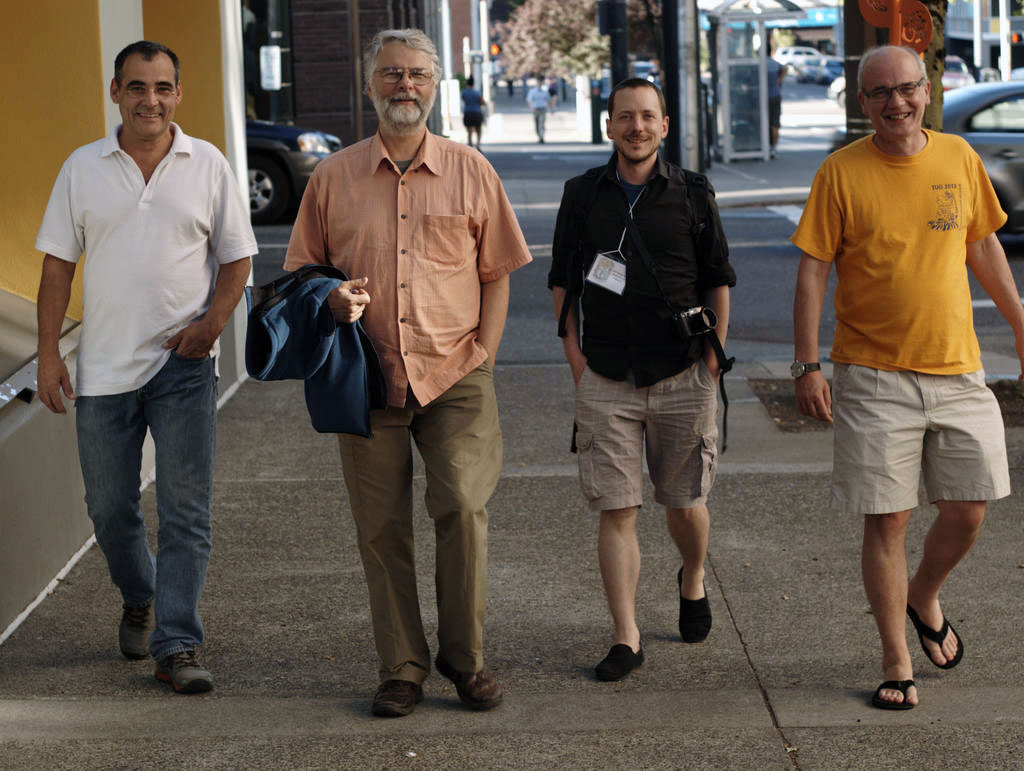
\includegraphics[width=\textwidth]{gangoffour.jpg}
      {\vskip-.75\baselineskip\hspace*{13pt}\hbox to \textwidth{\hfill\HUGE{6}\copyright Pavneet Arora}}
      \vfill
    \end{column}
    \begin{column}{.45\textwidth}
      \par\vspace*{-15pt}\hspace*{5pt}
      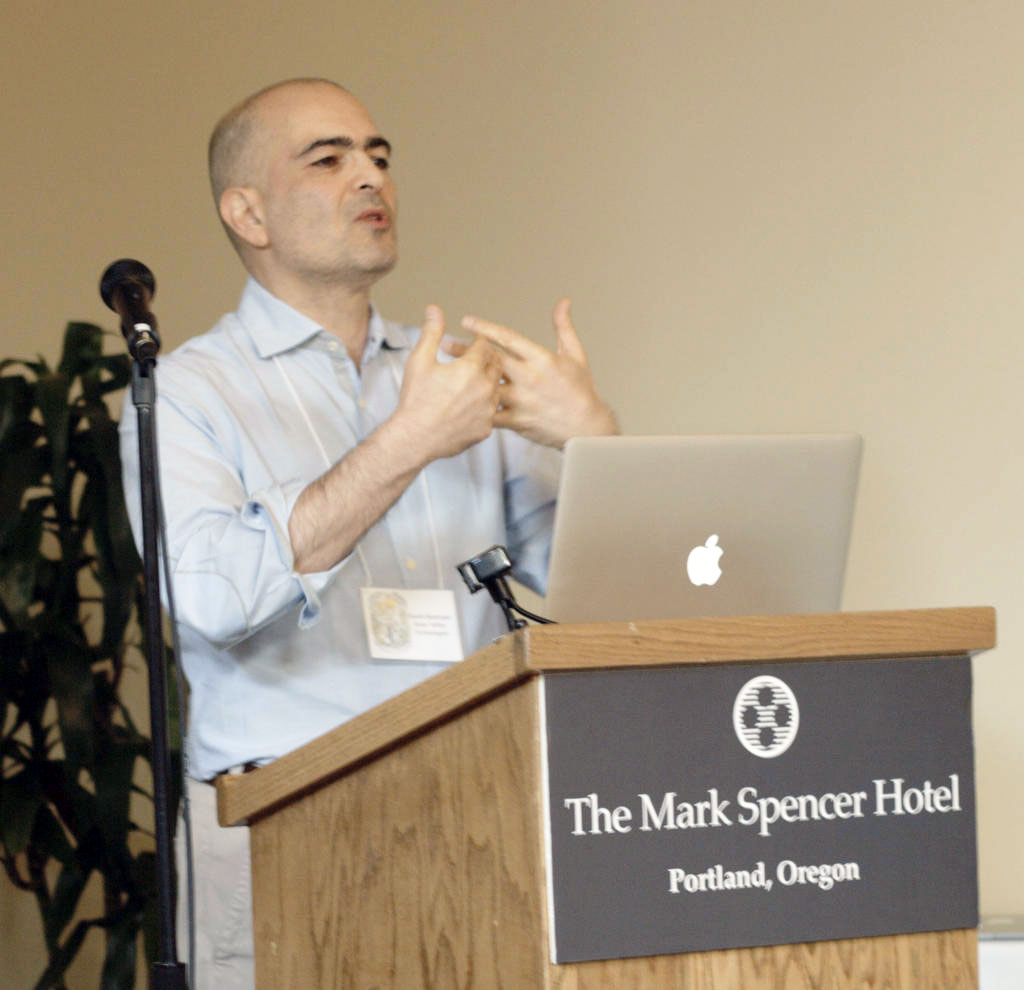
\includegraphics[width=.8\textwidth]{kaveh.jpg}
      {\vskip-.75\baselineskip\hspace*{9pt}\hbox to .8\textwidth{\hfill\HUGE{6}\copyright Pavneet Arora}}
    \end{column}
  \end{columns}
\end{frame}

\begin{frame}[t]{Most Interesting (for me)}
  \bfseries\rmfamily
  \begin{itemize}
    \item \TeX\ will be useful for non-printing media \\
    \begin{columns}[t]
      \begin{column}{.6\textwidth}
      \vspace{-20pt}\
      \setlength{\leftmarginii}{18pt}
      \begin{itemize}
        \item[] \begin{itemize}
        \item Reflowable PDFs
        \item Enhanced PDFs
        \item MathBook XML
        \item \LaTeX\ to MathML with CSS,\\ instead of MathJax
        \item \LaTeX\ to HTML, in the AIM journal
        \item Plotty, Wiki, ...
        \end{itemize}
      \end{itemize}
      \end{column}
      \begin{column}{.4\textwidth}
      \vspace{-40pt}
        \begin{columns}[t]
          \begin{column}{.7\textwidth}
            \par\vspace*{0pt}
            {\vskip-\baselineskip\hspace*{10pt}\HUGE{6}\copyright Pavneet Arora}
            \hspace*{10pt}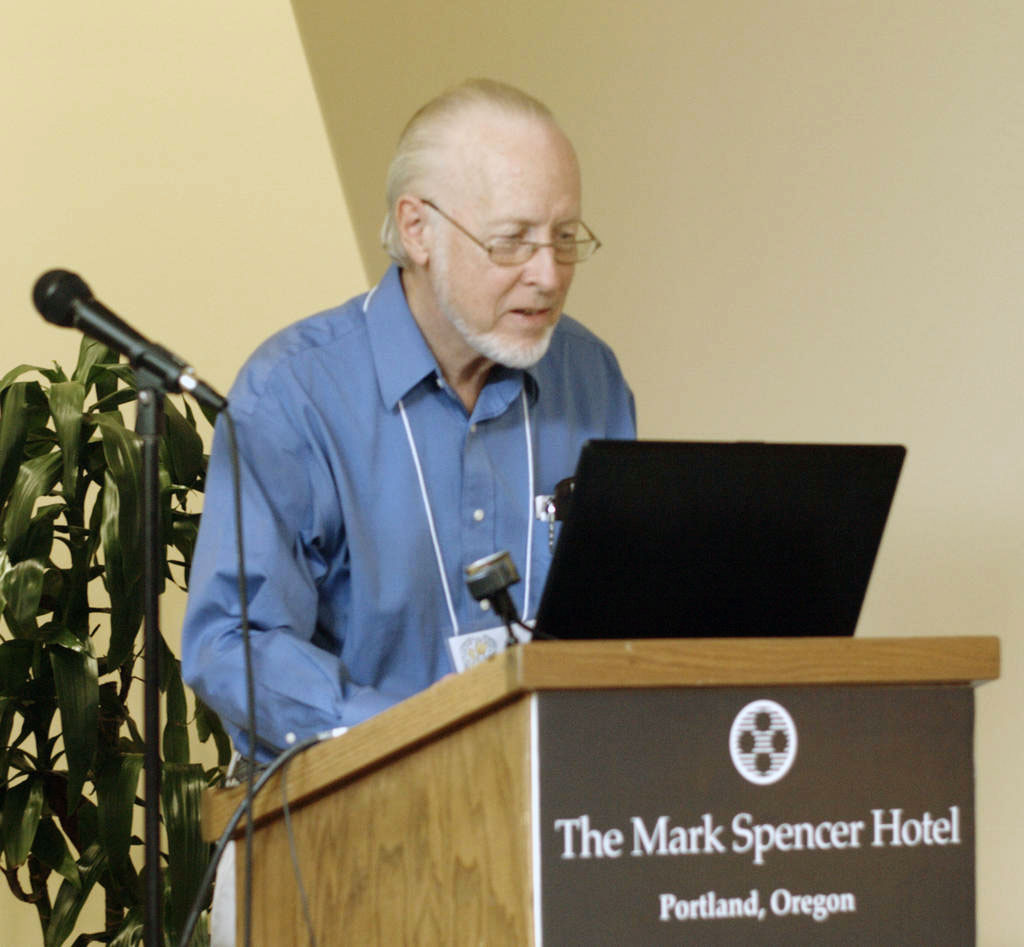
\includegraphics[width=\textwidth]{william.jpg}
            \vfill
          \end{column}
          \begin{column}{.7\textwidth}
            \par\vspace*{40pt}\hspace*{-40pt}
            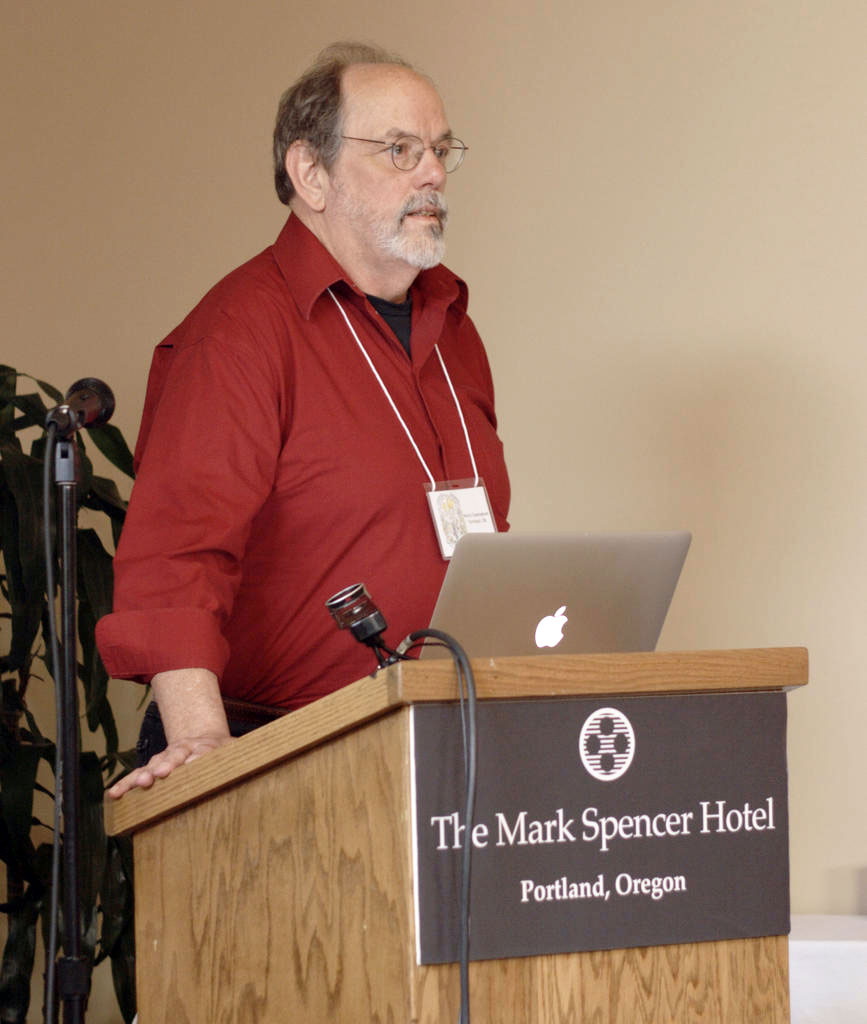
\includegraphics[width=.9\textwidth]{ward.jpg}
            {\vskip-.75\baselineskip\hspace*{-36pt}\hbox to .9\textwidth{\hfill\HUGE{6}\copyright Pavneet Arora}}
          \end{column}
        \end{columns}
      \end{column}
    \end{columns}
  \end{itemize}
\end{frame}

\begin{frame}[t]{Outside of the Presentations}
  \bfseries\rmfamily
  \begin{itemize}
    \item Lots of pleasant chat with friends !!\\
    \begin{columns}[t]
      \begin{column}{.4\textwidth}
      \vspace{-30pt}\
      \setlength{\leftmarginii}{32pt}
      \begin{itemize}
        \item[] \begin{itemize}
          \item lunchtime,
          \item banquet,
          \item breakfast, 
          \item and nightlife
        \end{itemize}
      \end{itemize}
        \par\vspace*{12pt}\hspace*{20pt}
        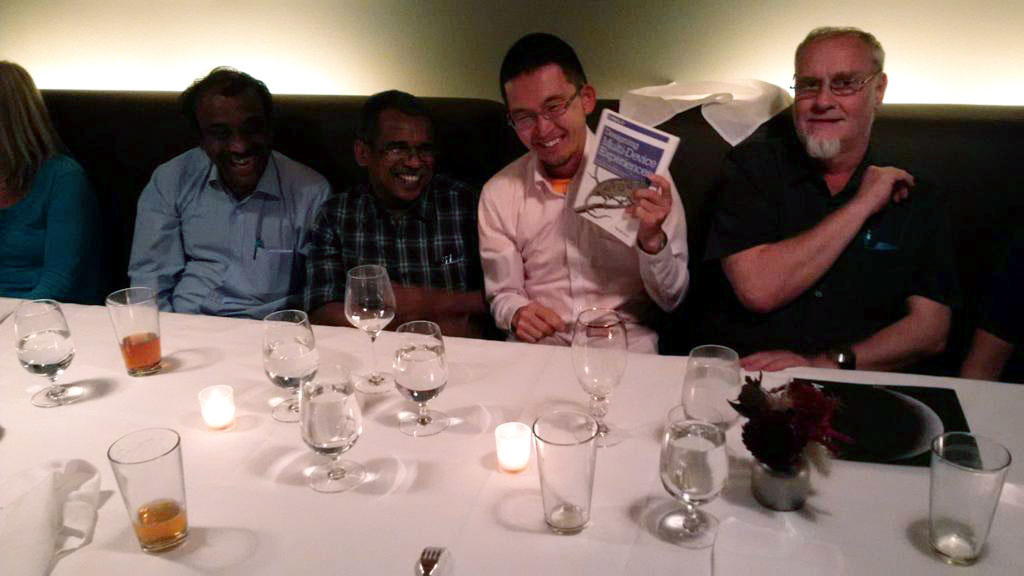
\includegraphics[width=.9\textwidth]{banquet.jpg}
        {\vskip-.75\baselineskip\hspace*{23pt}\hbox to .9\textwidth{\hfill\HUGE{6}\copyright Pavneet Arora}}
      \end{column}
      \begin{column}{.7\textwidth}
      \vspace{-33pt}
        \begin{columns}[t]
          \begin{column}{.4\textwidth}
            %\par\vspace*{0pt}\hspace*{0pt}
            {\vskip-\baselineskip\hspace*{10pt}\HUGE{6}\copyright Pavneet Arora}
            \hspace*{10pt}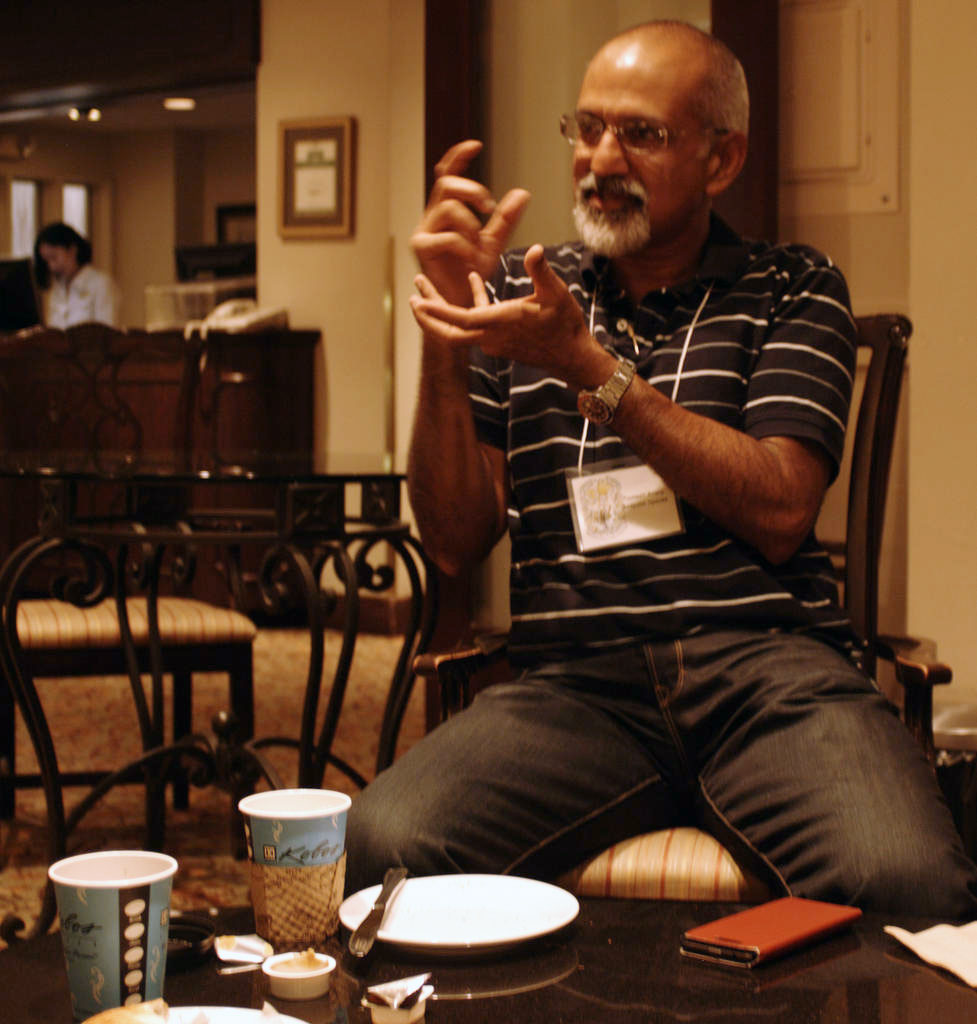
\includegraphics[width=.8\textwidth]{pavneet.jpg}
            \par\vspace*{0pt}\hspace*{0pt}
            \hspace*{6.8pt}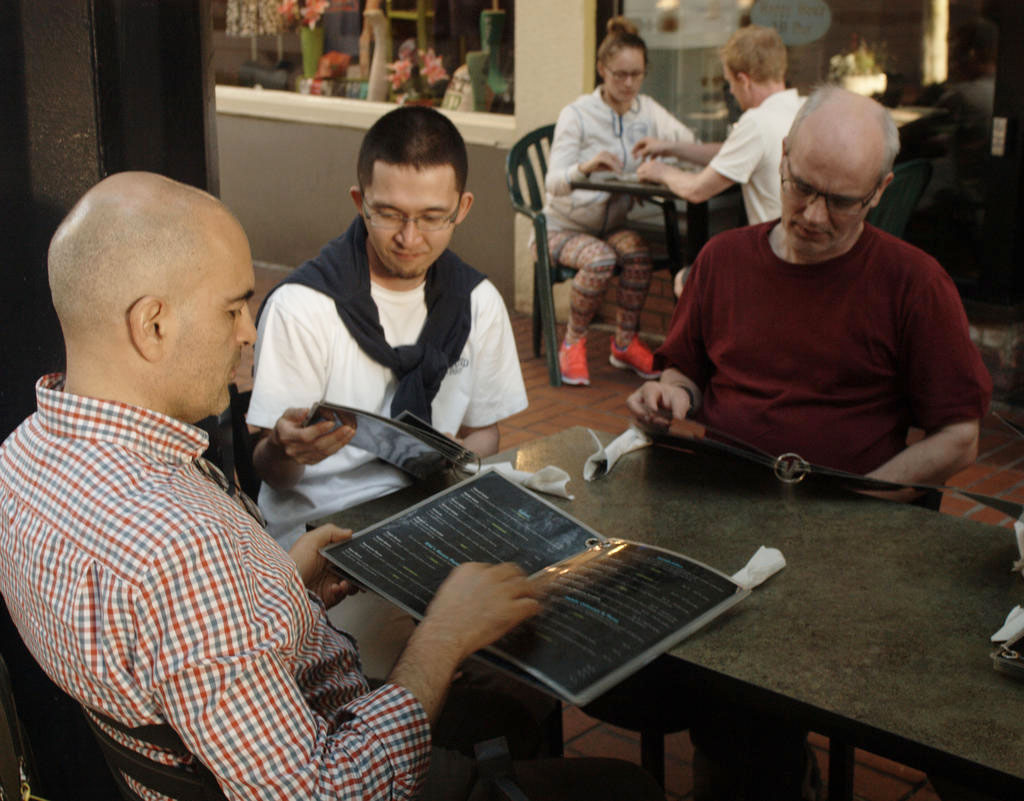
\includegraphics[width=.9\textwidth]{dinner.jpg}
            {\vskip-.75\baselineskip\hspace*{10pt}\hbox to .9\textwidth{\hfill\HUGE{6}\copyright Pavneet Arora}}
            \vfill
          \end{column}
          \begin{column}{.4\textwidth}
            {\vskip-\baselineskip\hspace*{-30pt}\HUGE{6}\copyright Pavneet Arora}
            \par\hspace*{-30pt}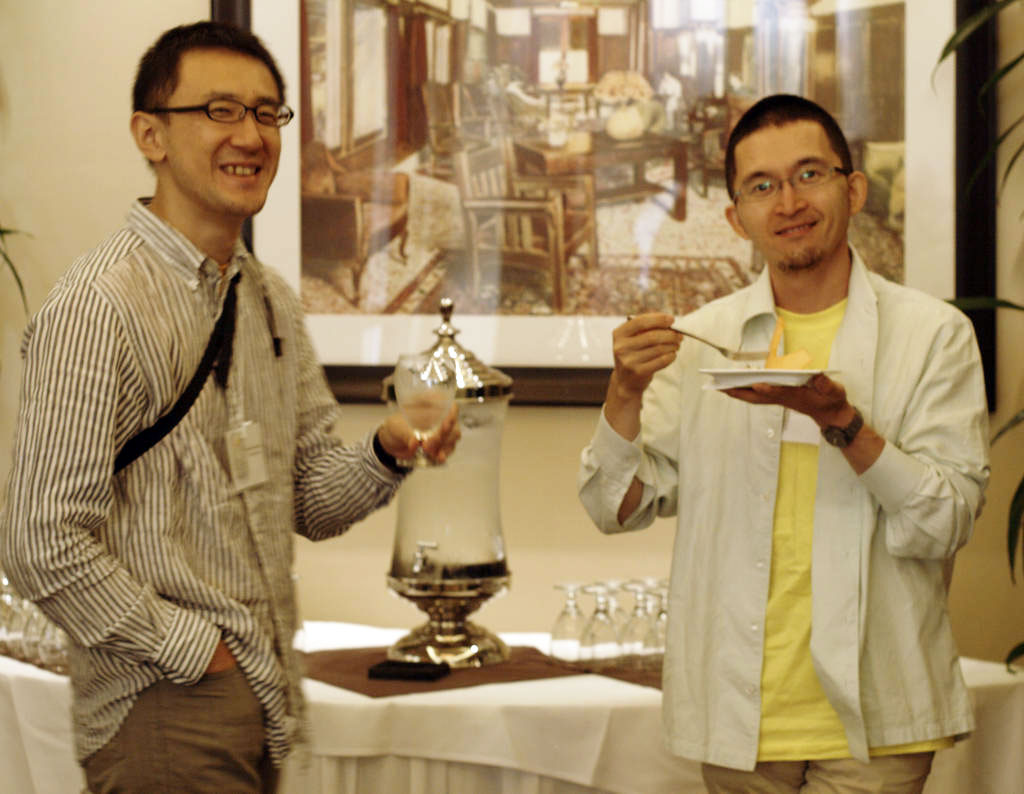
\includegraphics[width=.92\textwidth]{robby.jpg}
            \par\vspace*{0pt}\hspace*{-24pt}
            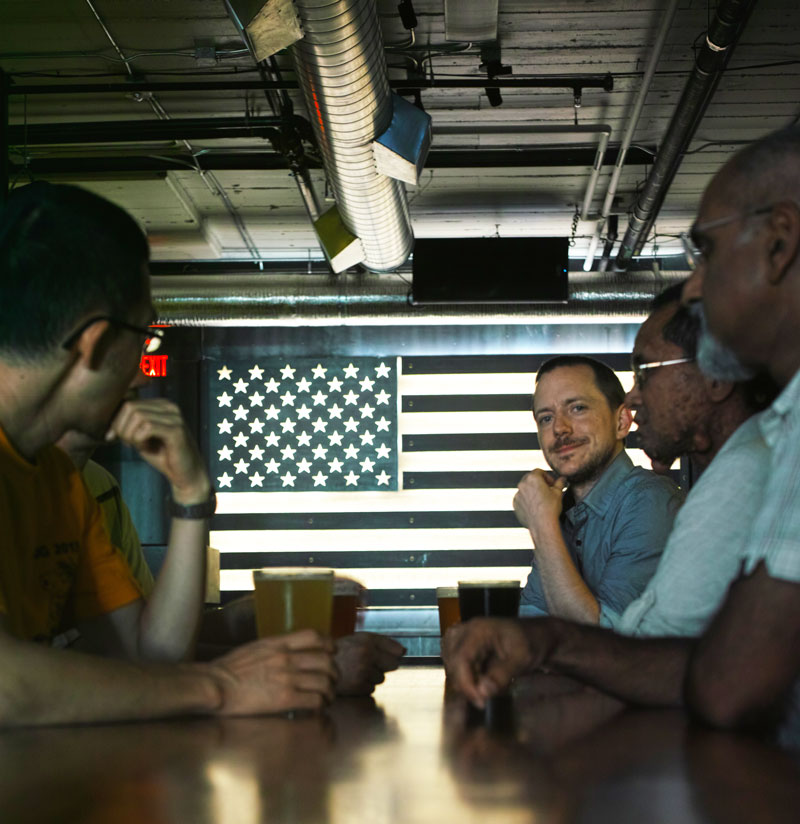
\includegraphics[width=.8\textwidth]{pub.jpg}
          \end{column}
        \end{columns}
      \end{column}
    \end{columns}
    \pause \item It's definitely the best part of TUG !
  \end{itemize}
\end{frame}

\begin{frame}[t]{Why don't you go, too?}
  \bfseries\rmfamily
  \begin{itemize}
    \item TUG 2015 will be held in Darmstadt, Germany on July 20 -- 22
    \item No need to prepare a presentation
    \pause \item Just visit and drink beer!
  \end{itemize}
  \begin{center}
    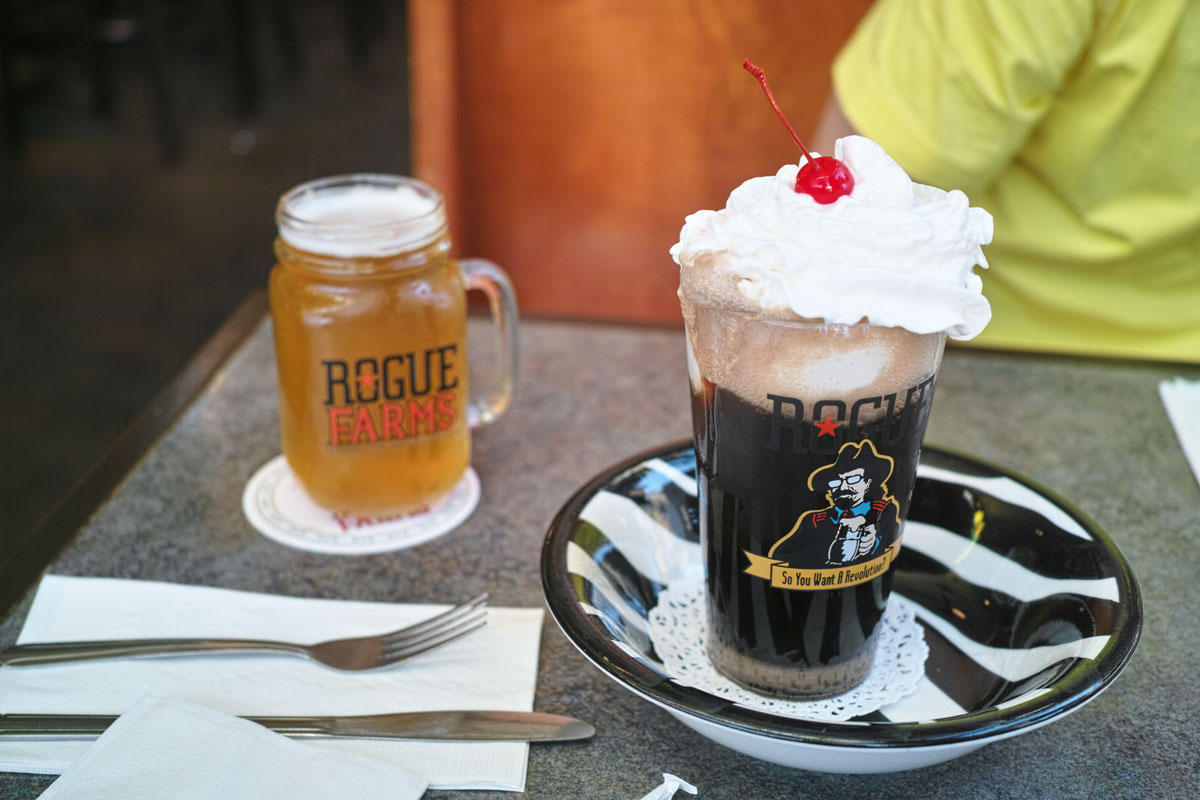
\includegraphics[width=.55\textwidth]{creambeer.jpg}
  \end{center}
\end{frame}

\end{document}

